\selectlanguage{italian}
\chapter{Introduzione parte II}
Questa parte di corso si concentra sul condurre inferenza su i dati disponibili.
In particolare, la statistica classica ci può aiutare a trovare correlazione tra i dati,
ci avverte che correlazione non è causalità\sidenote[][-0.8cm]{Per esempio, se i lavoratori $L$ di 
un'azienda sono proporzionali al fatturato $F$ tramite una costante di proporzionalità $k$
, allora $L = kF$, $L - kF = 0$ e $F = L/k$ sono tutte corrette, non abbiamo informazioni
su quale sia il driver, se il fatturato o il numero di lavoratori.}, ma non ci dice quale 
sia la causa di un fenomeno e come si identifica.
Le risposte a queste domande non risiedono nei meri dati.
\begin{figure*}
    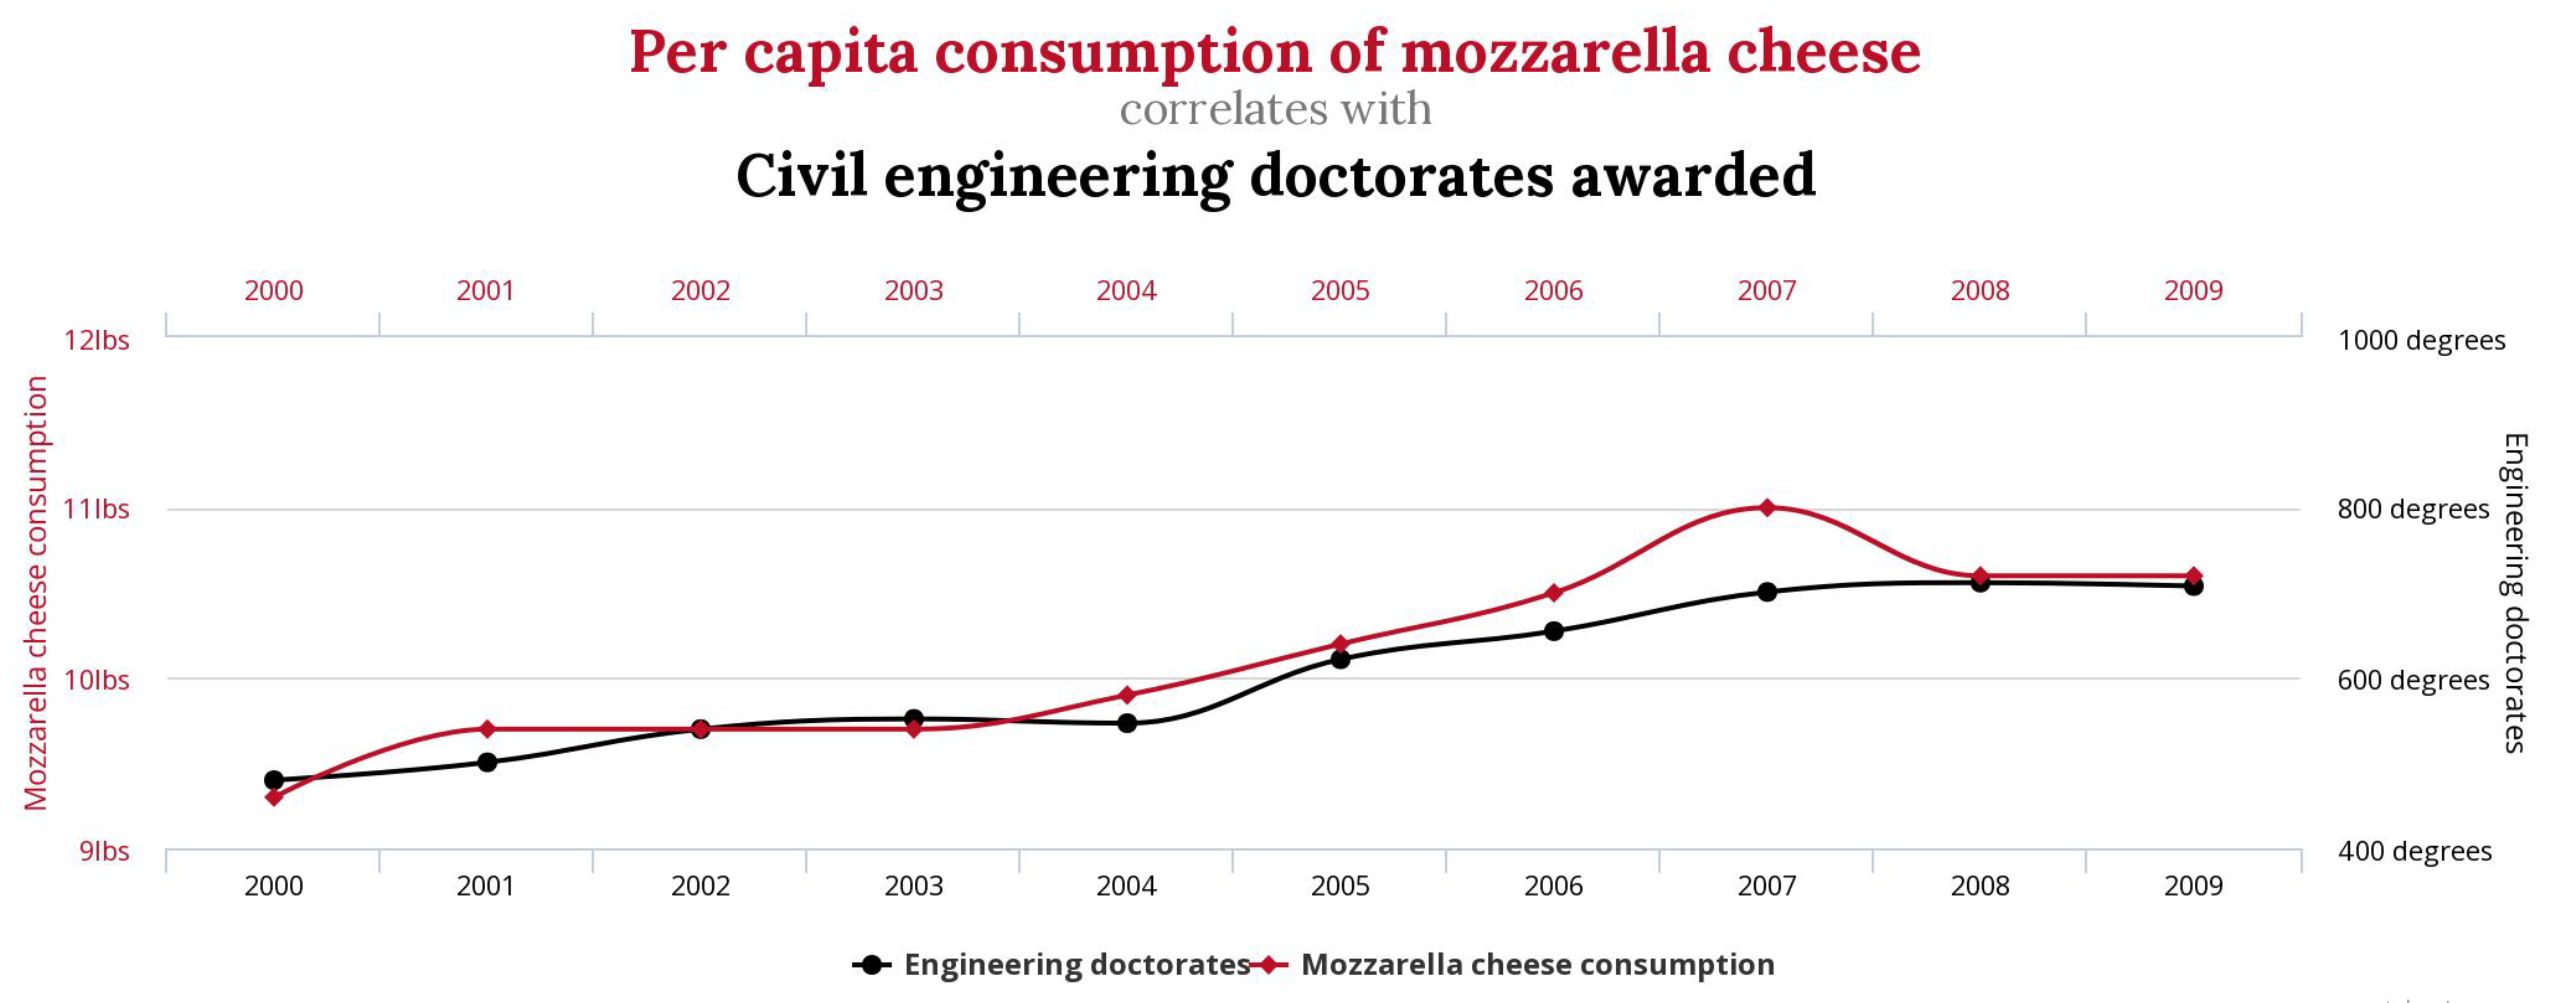
\includegraphics[width=\textwidth]{mozzarella}
\end{figure*}
\\ Correlazione significa co-variabilità: variabili correlate tendono a variare assieme.
La causalità implica una relazione tra due variabili di cui una è causa dell'altra.
Si noti che la correlazione è condizione necessaria ma non sufficiente per la causalità.

\section{Ceteris Paribus Condition}
Prendiamo come esempio l'analisi tra il debito sottoscritto dagli studenti e i loro risultati
accademici, e supponiamo di trovare una correlazione negativa.
Supporre allora che il debito abbia un'influenza negativa sulla performance accademica degli
studenti può essere fuorviante: il fatto che lo studente venga da una famiglia meno abbiente
può infatti essere ragionevolmente la causa di ambi i fenomeni. 
Questo vuol dire che il confronto non è \textit{a parità di condizioni} i.e. \textit{ceteris paribus}.
Il problema principale dell'inferenza nasce dal fatto che non possiamo confrontare i risultati
accademici degli stessi studenti se si indebitassero o meno.
L'econometria cerca quindi di costruire situazioni simili ad hoc, ovvero usa i dati per trovarsi
il più possibile nella situazione di "a pari condizioni", in modo da evitare i problemi che 
possono generare stime scorrette dell'effetto causale. Questo lavoro sui dati viene descritto 
dal \textit{do operator}.

\section{Do Operator}
Immaginiamo di predirre $Y$ usando $X$ su certi dati osservazionali. In generale
\begin{equation}
   P(Y | X) = \frac{P(X,Y)}{P(X)}
\end{equation}
Questa non è però una relazione causale, ma solo condizionata. Occorre dunque introdurre
il do operator, condizionando quindi anziché su $X$ su $\mathrm{do}(X)$.
In altre parole, dovremmo calcolare $P(Y | \mathrm{do}(X))$, che è la distribuzione condizionata
di $Y$ se fossimo in grado di intervenire nel processo di generazione dei dati e imporre 
$X = x$.
